\section{Evaluation: Modularity Index $Q_M$}\label{ev_metric}
In this section, we evaluate the proposed multilayer modularity $Q_M$ against baseline indices. In this experiment, we implement
different configurations of multilayer network following section~\ref{syn_gen} and regulate the tuning parameters to obtain
the desired topology.

\subsection{Baseline Multilayer Modularities}
In literature, very few modularity indices are proposed for multilayer networks, illustrated in~\cite{CompMod} \& \cite{medical_paper}.
Out of this two, `CompMod' proposed in~\cite{CompMod}
works only for communities with single type of nodes (i.e. single layer communities), leaving us with only the modularity `mQ' proposed
in~\cite{medical_paper} to compare with $Q_M$.
For a two-layer network $\mathcal{G} = \{\{L_1, L_2\}, \{L_{12}\}\}$ where $L_1$ = ($V_1$, $E_1$) \& $L_2$ = ($V_2$, $E_2$) are the
individual layers and $L_{12}$ = ($V_1$, $V_2$, $E_{12}$) is the bipartite graph connecting nodes of layer $L_1$ and $L_2$,
$mQ$ can be defined as, %[BM: correct C in the eq.]
\vspace{-0.1in}
\begin{dmath}\label{eq_mQ}
%\resizebox{\columnwidth}{!}{
 {mQ=\frac{1}{3}\sum_{k=1}^{n_C} \bigg \{
 \underbrace{\big(\frac{\left \vert E^{C_k}_1 \right \vert}{\left \vert E_1 \right \vert}-
 (\frac{h^{C_k}_1}{2\left \vert E_1 \right \vert})^2\big)}_{Term~ for~ Single~ Layer~ L_1}}
 +{\underbrace{\big(\frac{\left \vert E^{C_k}_{12} \right \vert}{\left \vert E_{12} \right \vert}-
 \frac{r^{C_k}_{12}*{s^{C_k}_{12}}}{{\left \vert E_{12} \right \vert}^2}\big)}_{Term~ for~ Coupling~ Edges}
 +\underbrace{\big(\frac{\left \vert E^{C_k}_2 \right \vert}{\left \vert E_2 \right \vert}-(\frac{h^{C_k}_2}{2\left \vert
 E_2 \right \vert})^2\big)}_{Term~ for~ Single~ Layer~ L_2} \bigg\}}
 %}
\end{dmath}
\vspace{-0.1in}
%[BM: with underbrace, write - term for single layer $L_1$, term for crosslayer edges, term for single layer $L_2$]
where each community ${C_k}$ 
%[BM: make suitable changes in notation here] 
is represented as $\{\{L^{C_k}_1, L^{C_k}_2\}, 
\{L^{C_k}_{12}\}\}$;
$L^{C_k}_1$ and $L^{C_k}_2$ are the submodules with $E^{C_k}_1$ \& $E^{C_k}_2$ edges from $E_1$ and $E_2$ respectively
whereas $L^{C_k}_{12}$ contains $E^{C_k}_{12}$ edges from $E_{12}$;
%$I^C_1$ is the number of edges in submodule $L^C_1$ i.e. $I^C_1 = \left \vert E^C_1 \right \vert$,
%$m_1$ is the size of subnetwork $G_1$ i.e. ,
$n_C$ is the number of apriori communities; $h^{C_k}_i$ is the sum of degrees of all $L^{C_k}_i$ nodes in $L_i$ layer;
$r^{C_k}_{12}$ is the sum of degrees of $L^{C_k}_1$ nodes in subnetwork $L_{12}$ and $s^{C_k}_{12}$ is the sum of
degrees of $L^{C_k}_2$ nodes in subnetwork $L_{12}$.
% In fact, this definition is basically a linear combination of Newman-Girvan modularity for simple graph~\cite{newman2004finding}
% and Barber modularity for bipartite graph~\cite{barber2007modularity}.

\subsection{Network configurations}
In order to compare $mQ$ and $Q_M$, we construct a synthetic two-layer network $\{\{L_1, L_2\}, \{L_{12}\}\}$ (see Fig.~\ref{N0}) with
three cohesive groups of same type of nodes (cliques) at each
layer $L_1$ and $L_2$ respectively. Each clique contains $100$ nodes (hence, $300$ nodes per layer) and each layer contains 
$14,852$ intra layer edges.
%[BM: one line on number of nodes, links etc.] 
We consider two typical ground truth community configurations
as shown in Fig.~\ref{N0} - (i) \textbf{Config A:} single-layer communities comprising cohesive groups of single type of nodes
only (six communities),
(ii) \textbf{Config B:} cross layer communities, each comprising one group of nodes from Layer $L_1$ with another group from
layer $L_2$ (three communities). Importantly, coupling edges, connecting two types of nodes, are the key characteristics of
the multilayer network, which makes it strikingly different from multiplex network. Hence in this evaluation, we primarily
concentrate on the coupling edges as a regulating topological parameter.
The coupling edges between layers $L_1$ and $L_2$ can be tuned by varying the density parameters $d$ and $p$ (as discussed in 
section~\ref{syn_gen}).


% \begin{figure}
% \centering
% 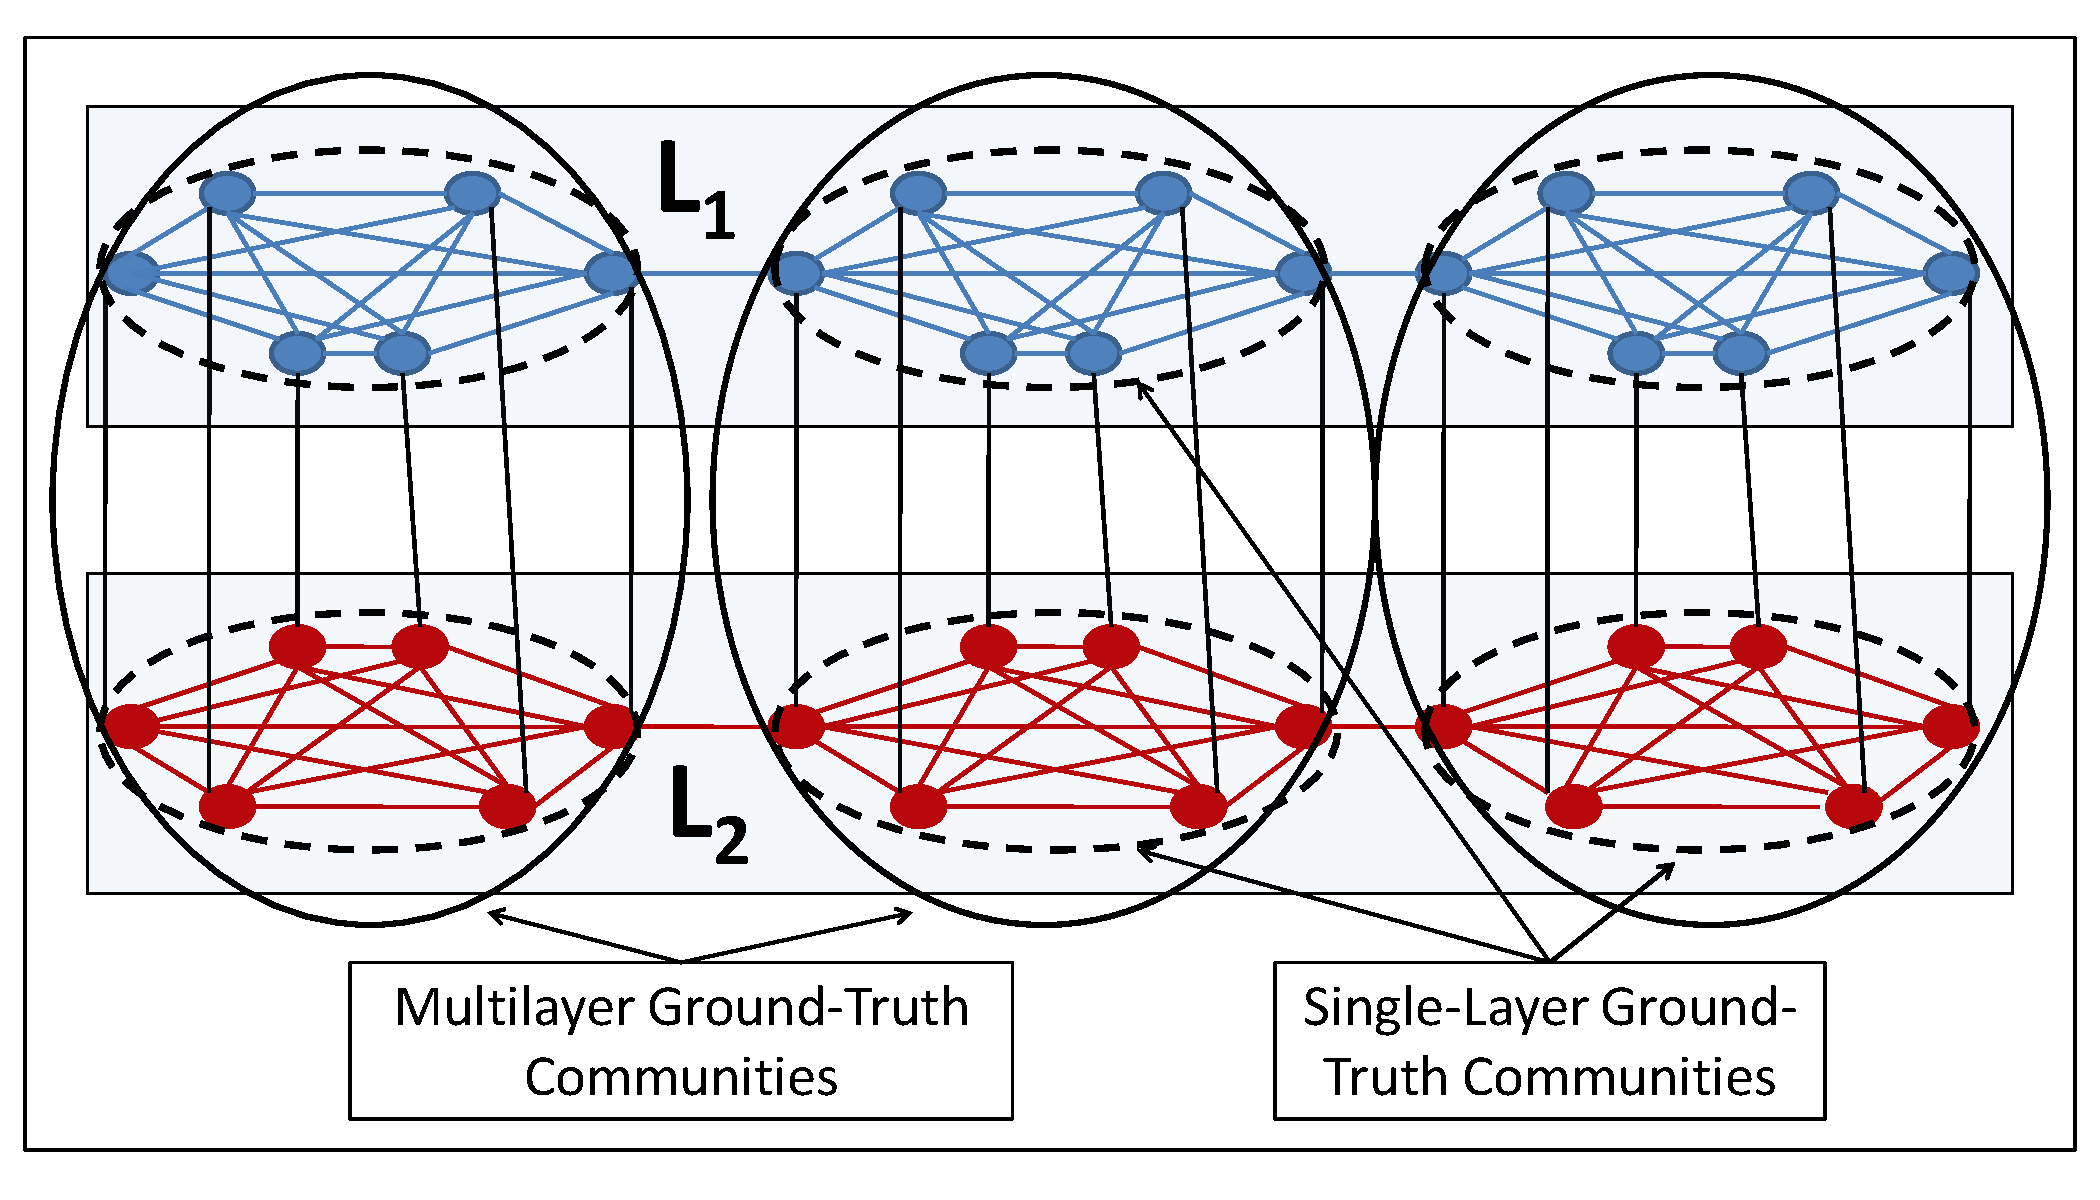
\includegraphics[width=2.5in]{./images/image31.pdf}
% \vspace{-0.1in}
% \caption{Network configuration with two different ground truth communities}
% \label{N0}
% \end{figure}

\subsection{Experimental Results}
In our experiment, we increase the coupling edge density $d$ from $0$ to $1$, for both the ground truth configurations A \& B,
with different $p$ values.
Intuitively, addition of coupling edges should dilute the single layer community structures in Config A, decreasing the
modularity of Config A, whereas in Config B, it should make the cross layer
communities more cohesive, increasing the modularity.

\subsubsection{Config A}
In Fig.~\ref{cross_single} the plot corresponding to $mQ$ reveals that it is completely insensitive 
to the increase in
coupling edge density $d$. Precisely, in case of Config A the coupling edges
do not have any contribution in Eq.~\ref{eq_mQ} (coupling edge term vanishes for single layer communities),
hence $mQ$ remains invariant against addition of
coupling edges. On the contrary, in case of $Q_M$, we penalize for the coupling edges connected with single layer
communities (see $(h_i+\theta_{C_k}*c_i)$ terms in Eq.~\ref{final1}) which allows us to achieve the drop in $Q_M$ values with 
increasing $d$ (see
Fig.~\ref{cross_single}). This result concurs with the desired $Property^S$, introduced in section~\ref{prop}. 
%Config A does not have any cross layer community; so both the plots in Fig.~\ref{cross_single} are invariant with $p$.

% \begin{figure}
% \centering
% 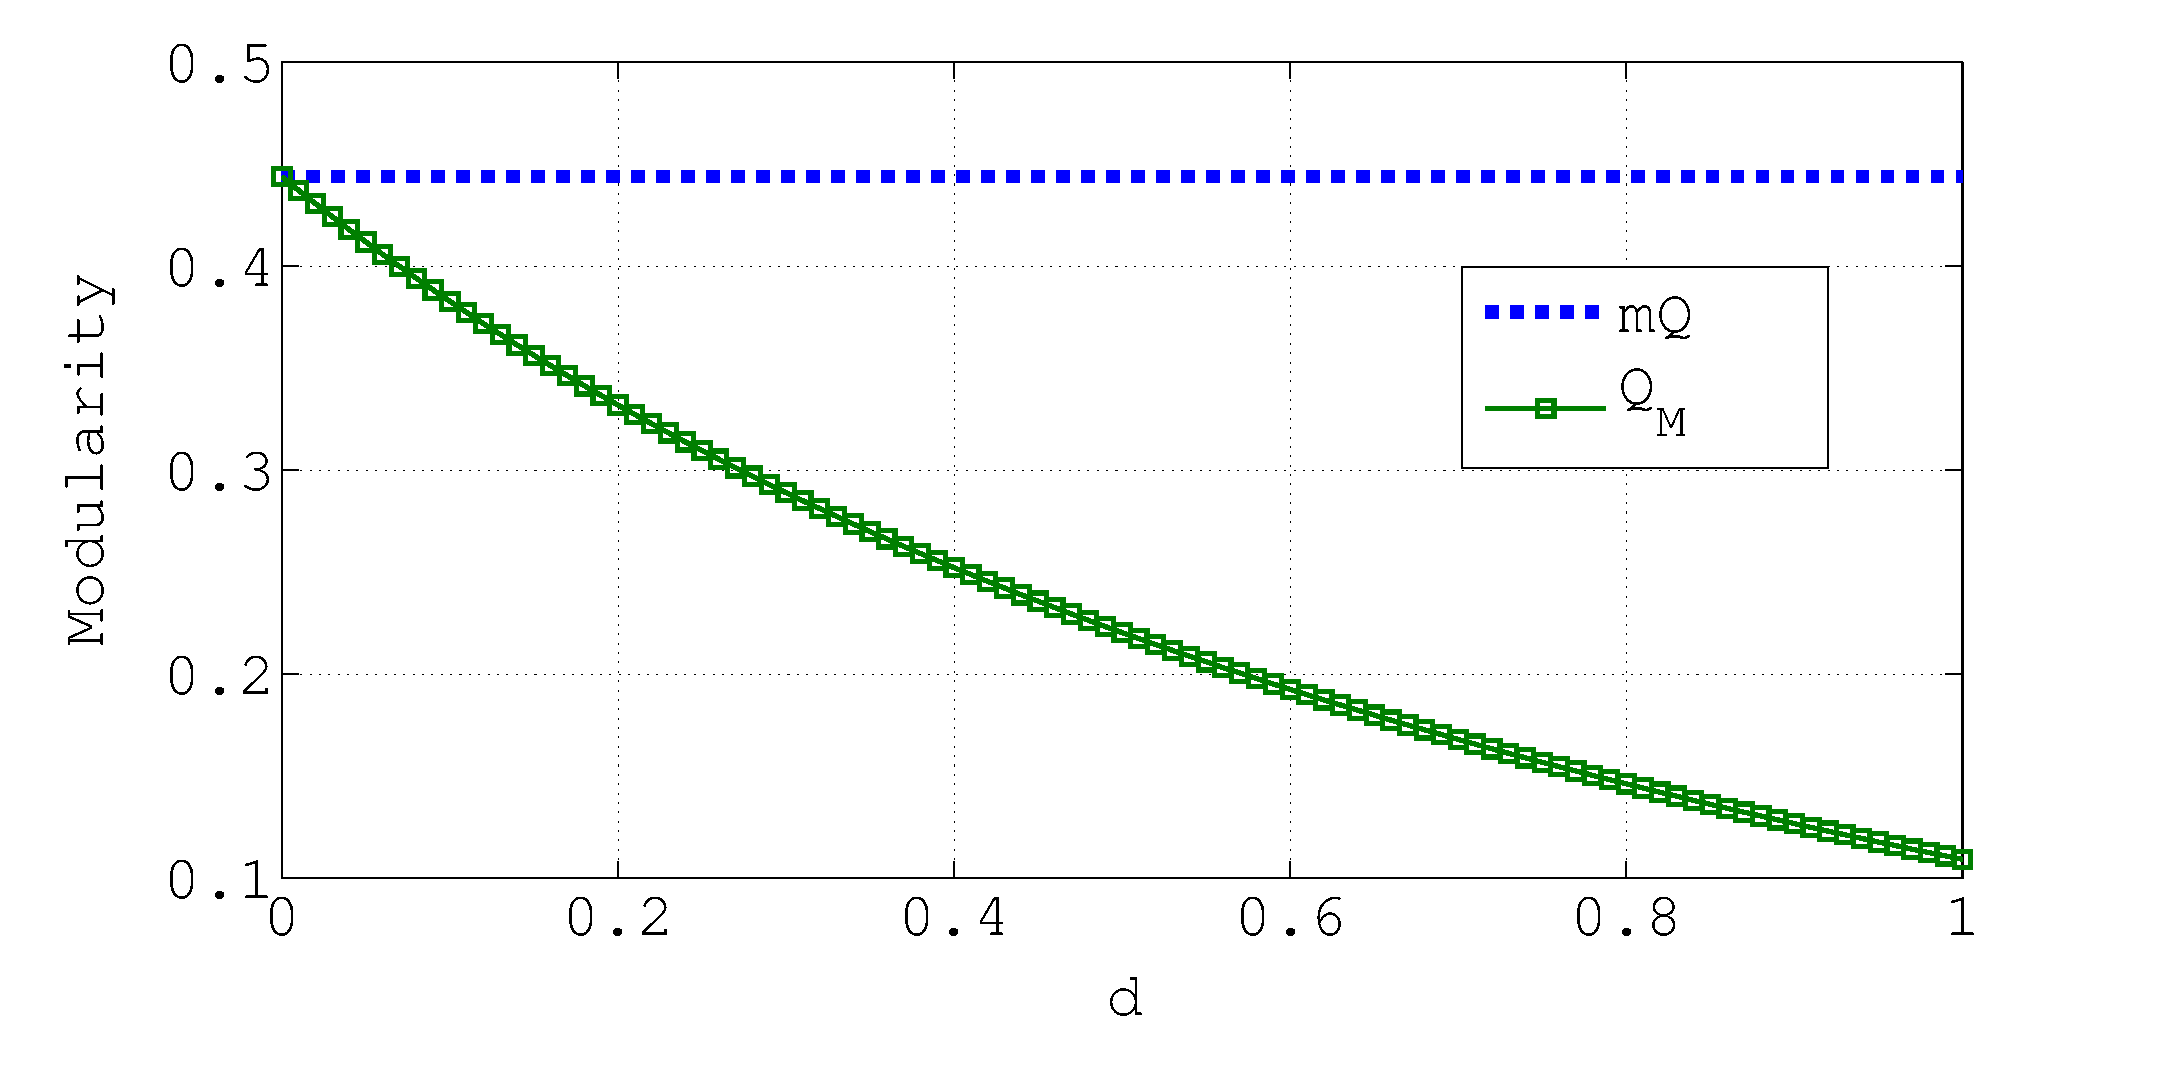
\includegraphics[width=2.5in]{./images/mQ_vs_march21_cross_single.pdf}
% \vspace{-0.1in}
% \caption{Comparison of $mQ$ and $Q_M$ for Config A while adding coupling edges with different $P$ values}
% \label{cross_single}
% \end{figure}

\subsubsection{Config B}
In case of Config B, $mQ$ is unable to capture the desired increasing behavior (see $Property^X$, introduced in section~\ref{prop}) with
the increase in coupling edges (except at
the beginning when $d$ becomes non-zero for the first time). Rather, it remains constant throughout the edge addition
regime irrespective of the $p$ values (see Fig.~\ref{cross_multi}).
In Config B, as observed from Eq.~\ref{eq_mQ}, the coupling edge addition only affects the 
term for coupling edges
%bipartite modularity term [BM: what is this term in eq 7? term for coupling edges? Then write it directly] 
of $mQ$;
however, addition of edges influences the numerator and denominator almost equally, neutralizing the overall effect on $mQ$.
%Essentially, here the major deficiency of modularity $mQ$ stems from the fact that it evaluates the quality of a cross layer community
%by individually checking its single layer and bipartite components without verifying how well the individual single layer components within each cross layer community are connected with each other.
On the other hand, in all the plots corresponding to $Q_M$, the modularity increases gracefully with coupling
edge addition. This is achieved by suitably penalizing the null model in Eq.~\ref{eq_multi}.
%This is due to the consideration of intra layer degrees of nodes which are not connected via coupling edges in the middle term of $Q_M$ (see Eq.~\ref{final1}) which helps to penalize the bipartite modularity for having such nodes in the community.
As expected, the absolute value of modularity increases with $p$ for both $mQ$ and $Q_M$, since higher $p$ improves the cohesiveness
of cross layer communities.

% \begin{figure}
% \centering
% 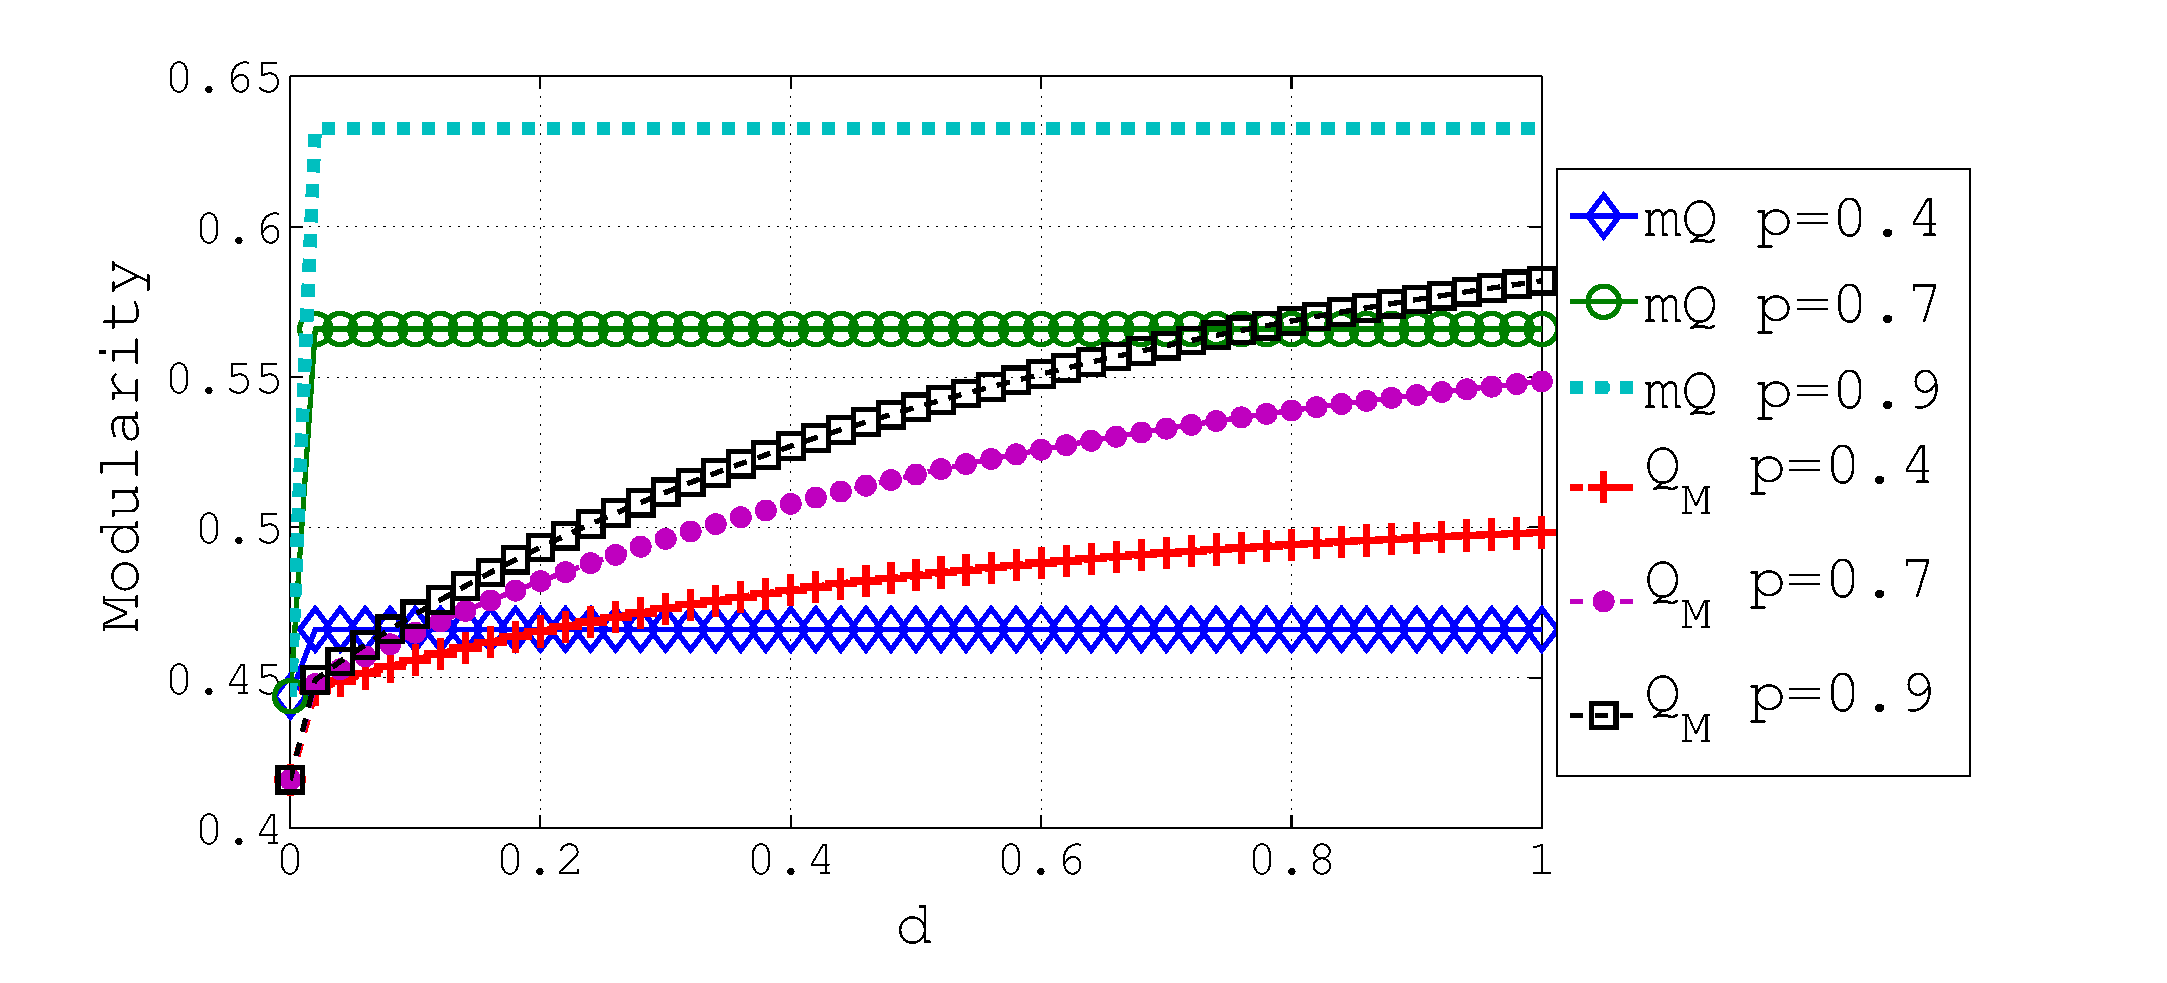
\includegraphics[width=3.5in]{./images/mQ_vs_march21_cross_multi.pdf}
% \vspace{-0.1in}
% \caption{Comparison of $mQ$ and $Q_M$ for Config B while adding coupling edges with different $P$ values}
% \label{cross_multi}
% \end{figure}

In a nutshell, the aforesaid experiments clearly demonstrate the elegance of $Q_M$ with respect to $mQ$, as a community quality index.
%In the next two sections, we evaluate how efficiently we can discover communities with the help of $Q_M$ in synthetic and empirical multilater networks.

% % We illustrate this limitation with the help of a representative example.
% % (a) We introduce the factors $e^{-F^C_1}$ and $e^{-F^C_2}$, respectively with the corresponding single layer modularity terms.
% % Consider a community $L^C_1$ which is very cohesive in the $L_1$ layer itself, however a high fraction of
% % nodes in $L^C_1$ may also be connected with the nodes of some different community of layer $L_2$ through coupling
% % edges (high $F^C_1$); this should dilute the cohesiveness of community $L^C_1$ and penalize the overall modularity.
% % Hence, we introduce the factors $e^{-F^C_1}$ and $e^{-F^C_2}$ to penalize the single layer terms of modularity.
% % Fig.~\ref{single1} depicts that in Config A, modularity
% % $MultiMod$ gracefully improves as a result of removal of these type of coupling edges.
% %
% % (b) The factor $H^C_1\times H^C_2$, introduced with the coupling layer term of Eq.~\ref{eqn2}, measures how strongly the coupling
% % edges in community $C$ connect the group of nodes
% % $L^C_1$ and $L^C_2$ respectively. In Config B, even if the cross layer term results in high modularity, removal
% % of coupling edges results in low $H^C_1\times H^C_2$, which in turn reduces $MultiMod$. In Fig.~\ref{single0}, we can
% % observe that in Config B, $MultiMod$ gracefully degrades, following our intuition, with deletion
% % of coupling edges.



%\subsection{Ranking Algorithms}



%\subsection{Sensitivity} 